\begin{frame}
    \frametitle{前情回顾}
    \begin{itemize}
        \item 光场量子化~~真空态~~数态~~产生湮灭算符 
        \item 相干态~~压缩态~~辐射场 
        \item 光子计数 ~~ 关联函数~~反聚束
        \item 光场表象
    \end{itemize}     
\end{frame}

%%%%%%%%%%%%%%%%%%%%%%%%%%%%%%%%%%
\begin{frame} [plain]
    \frametitle{}
    \Background[1] 
    \begin{center}
    {\huge 第16-17讲:光与原子的相互作用}
    \end{center}  
    \addtocounter{framenumber}{-1}   
\end{frame}



\begin{frame} 
\frametitle{}
{\Bullet}光与物质相互作用在光谱学、传感、催化、量子信息学和激光等领域发挥着重要作用。通常光被视为电磁平面波,与物质的相互作用可视为非常弱,在量子电动力学中只考虑低阶项。\\
  \begin{center}
       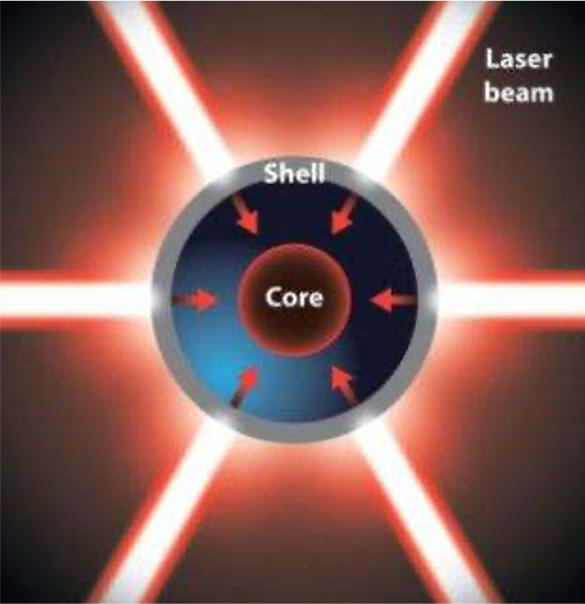
\includegraphics[width=0.2\textwidth]{figs/23.png}
  \end{center}
{\Bullet}当光被限制在微小区域区域(尺度与波长相当)时,不能被视为平面波. 具体丰富的量子化效应。
\end{frame}

\section{1. 光-原子系统的哈密顿}

\begin{frame} 
 \frametitle{}
 \begin{tcolorbox2}[1.0]{哈密顿}
    量子力学的核心是薛定谔方程;最重要是给出正确的哈密顿; 如果哈密顿错了,一切都错了.正确的H量是所有工作的基础。
  \end{tcolorbox2}
 光场含时, 体系服从含时薛定谔方程
      \[ i \hbar \frac{\partial \psi}{\partial t} = H \psi \]
      哈密顿分解成原子哈密顿$H_S$, 光场哈密顿 $H_F(t)$和光与原子相互作用$H_I(t)$三项
      \[H= H_S+H_F+H_I(t) \]
\end{frame}

\begin{frame} 
\frametitle{}
    ~\\
      {\Bullet}真空中,原子的哈密顿 $H_S$ 可分解成四部分:
     \[ H_S = H_c + \sum H_e + \sum H_{ce} + \sum H_{ee}\]
     分别为核的动能$H_c$ , 电子的动能$H_e$, 电子与核的的相互作用能$H_{ce}$, 电子与电子的相互作用能$H_{ee}$. \\ {\vspace*{0.3em}}
     若不含时,决定了薛定谔方程的解为:
      \[ \psi_n(\mathbf{r},t)= \psi_n(\mathbf{r})e ^{-i E_n t/\hbar} \]
    基中, $\psi_n(\mathbf{r})$, 是能量本征解
\end{frame}

\begin{frame} 
 \frametitle{}
 {\Bullet} 光场哈密顿$H_F(t)$可做模式分解
 \[ H_F(t)= \sum_{k,\sigma}\hbar \omega_{k\sigma} \left(\hat{a}^\dagger _{k\sigma} \hat{a} _{k\sigma}+ \frac{1 }{2}\right) \qquad \text{with} \quad [\hat{a} _{k\sigma},\hat{a}^\dagger _{k\sigma}]=1 \]
 解的具体形式由限域边界条件决定. \\ {\vspace*{2.3em}}
 
 比如, 一维单模腔场解为:
 \[\begin{aligned}
   \hat{\mathbf{E}}_{x,l}( z,t) =& \sqrt{\frac{\hbar\omega_l}{ 2\epsilon_0 L }} (\hat{a}_l(t)+ \hat{a}_l ^\dagger(t)) \sin(k_l z) \\ =&E^0 _l (\hat{a}_l(t)+ \hat{a}_l ^\dagger(t)) E_l(z)\\
   \end{aligned} 
   \]
\end{frame}

\begin{frame} 
\frametitle{}
{\Bullet} 相互作用项$H_I(t)$可理解为原子的电子云密度($\rho(\mathbf{r})$)对光场势($\Phi(\mathbf{r})$)的积分
    \[ H_I = \int_V d^3 \mathbf{r} \rho(\mathbf{r}) \Phi(\mathbf{r})\]
    式中, V是相互作用所发生的体积.\\ {\vspace*{0.3em}} 
    把$\Phi(\mathbf{r})$泰勒展开
    \[\begin{aligned}
        \Phi(\mathbf{r}) &= \Phi(0) + \mathbf{r}\cdot \nabla \Phi(0) + \frac{1}{2} \sum_{i,j} r_i r_j \frac{\partial^2 }{\partial r_i \partial r_j }\Phi(0) + \cdots , \\ 
        &= \Phi(0) - \mathbf{r}\cdot \mathbf{E}(0) - \frac{1}{2} \sum_{i,j} r_i r_j \frac{\partial }{\partial r_i }E_j(0) + \cdots , \\ 
        &= \Phi(0) - \mathbf{r}\cdot \mathbf{E}(0) - \frac{1}{6} \sum_{i,j} (3r_i r_j-r^2\delta_ij) \frac{\partial }{\partial r_i }E_j(0) + \cdots , \\ 
        &= \Phi(0) - \mathbf{r}\cdot \mathbf{E}(0) - \frac{1}{6} \sum_{i,j} Q_{ij}\frac{\partial }{\partial r_i }E_j(0) + \cdots , \\ 
    \end{aligned} \]
    代回, 得
\end{frame}

\begin{frame} 
\frametitle{}
    \[ H_I = q\Phi(0) - q\mathbf{r}\cdot \mathbf{E}(0) - \frac{1}{6} \sum_{i,j} qQ_{ij}\frac{\partial }{\partial r_i }E_j(0) + \cdots \]
    \begin{enumerate}
        \item 第一项为电荷与光场势的相互作用
        \item 第二项为光场导致原子极化产生的偶极矩$\mu=q\mathbf{r}$与电场的相互作用
        \item 第三项为光场导致原子极化产生的四极矩与电场的相互作用
    \end{enumerate}
    通常,只考虑偶极相互作用. 
    \[ H_I = - q\mathbf{r}\cdot \mathbf{E}(0)\]
\end{frame}

\begin{frame} 
    \frametitle{}
    {\Bullet} 波恩近似下,可单列电子薛定谔方程
    \[ i \hbar \frac{\partial \psi}{\partial t} = H \psi \quad \cdots  (1)\]
    * 定域规范不变性(local guage invariance)导出的电子哈密顿:
    \[ H=-\frac{\hbar^{2}}{2 m}\left[\nabla-i \frac{e}{\hbar} \mathbf{A}(\mathbf{r}, t)\right]^{2}+e U(\mathbf{r}, t)+ H_{ec}\]
    光场的作用分解成矢势$\mathbf{A}$和标势$U$ 两项.  \\
    正确的H量要求定域规范变换条件下
    \[ \begin{aligned}
        \psi( \mathbf{r},t) & \to \psi( \mathbf{r},t)  e^ {i \chi(\mathbf{r}, t)}\\
        \mathbf{A}(\mathbf{r}, t)  & \to \mathbf{A}(\mathbf{r}, t)e^ {i \chi(\mathbf{r}, t)} \\
        U(\mathbf{r}, t) & \to U(\mathbf{r}, t) e^ {i \chi(\mathbf{r}, t)} 
    \end{aligned}\] 
    宏观物理量保持不变
\end{frame}

\begin{frame} 
\frametitle{}
    通常,电子哈密顿也可写成为
    \[ H(t)= H_e + H_{ec} + H_{eo}(t) = H_0 + H_I(t)\]
    光与原子相互作用表现为电子的跃迁(二能级). $H_0$决定的两能级的波函数为:
       \[ \psi_1(\mathbf{r},t)= \psi_1(\mathbf{r})e ^{-i E_1 t} \]
       \[ \psi_2(\mathbf{r},t)= \psi_2(\mathbf{r})e ^{-i E_2 t} \]
    空间函数是能量本征态:
       \[ H_0\psi_1(\mathbf{r})= E_1 \psi_1(\mathbf{r}) \]
       \[ H_0\psi_2(\mathbf{r})= E_2 \psi_2(\mathbf{r}) \]

\end{frame}

\section{2. 半经典理论}

\begin{frame} 
\frametitle{}
{\Bullet} 二能级系统的状态用叠加态描述
       \[ \begin{aligned}
          \psi(\mathbf{r},t) & = c_1 \psi_1(\mathbf{r})e ^{-i E_1 t /\hbar} + c_2 \psi_2(\mathbf{r})e ^{-i E_2 t \hbar}  \\
          &= c_1 \rs{1} e ^{-i \omega_1 t} + c_2 \rs{2} e ^{-i \omega_2 t}  \\
          &= c_1(t) \rs{1}  + c_2(t) \rs{2} \quad \cdots (2)
       \end{aligned}\] 
    存在
       \[ \left|c_1 \right|^2 + \left|c_2\right|^2 =1 \] 
{\Bullet} 二能级系统的哈密顿
    \[\begin{aligned}
    H_0 &= (\rs{1} \ls{1} + \rs{2} \ls{2})H_0(\rs{1} \ls{1} + \rs{2} \ls{2})    \\ 
    &= \hbar \omega_1 \rs{1} \ls{1} + \hbar \omega_2 \rs{2} \ls{2}  \quad \cdots (3)
    \end{aligned} \]    
\end{frame}

\begin{frame} 
\frametitle{}
    若光场用经典场描述, 偶极近似下光与原子的相互作用为:
    \[\begin{aligned}
       H_I(t) & = - e \mathbf{r}\cdot \mathbf{E}_0\cos \omega_0 t   \\
       &= - e  (\rs{1} \ls{1} + \rs{2} \ls{2}) \mathbf{r}(\rs{1} \ls{1} + \rs{2} \ls{2})\cdot \mathbf{E}_0\cos \omega_0 t  \\ 
       &= -e(\mathbf{r}_{12} \rs{1} \ls{2}+ \mathbf{r}_{21} \rs{2} \ls{1})\cdot \mathbf{E}_0\cos \omega_0 t \quad \cdots (4)
    \end{aligned} \]
    把(2)(3)(4)代回方程(1), 
    \[ \begin{aligned}
        i \hbar \frac{\partial }{\partial t} (c_1(t) \rs{1}  &+ c_2(t) \rs{2}) = (H_0 - e \mathbf{r}\cdot \mathbf{E}_0\cos \omega_0 t)   (c_1(t) \rs{1}  + c_2(t) \rs{2})\\
        &= (\hbar \omega_1 \rs{1} \ls{1} + \hbar \omega_2 \rs{2} \ls{2} - e(\mathbf{r}_{12} \rs{1} \ls{2}+ \mathbf{r}_{21} \rs{2} \ls{1})\cdot \mathbf{E}_0\cos \omega_0 t)\\ 
        &{\hspace*{2em}} \times (c_1(t) \rs{1}  + c_2(t) \rs{2})
    \end{aligned}\] 
    基于正交归一性,得关于展开系数的方程组... 
\end{frame}

\begin{frame} 
 \frametitle{}
 \[ \begin{cases}
    \frac{\mathrm{d}c_1(t)}{\mathrm{d}t}=\frac{\mathrm{i}}{2} \Omega_{\mathrm{R}}\left(\mathrm{e}^{\mathrm{i}\left(\omega-\omega_{0}\right) t}+\mathrm{e}^{-\mathrm{i}\left(\omega+\omega_{0}\right) t}\right) c_{2}(t) \\ 
    ~\\
    \frac{\mathrm{d}c_2(t)}{\mathrm{d}t}=\frac{\mathrm{i}}{2} \Omega_{\mathrm{R}}\left(\mathrm{e}^{-\mathrm{i}\left(\omega-\omega_{0}\right) t}+\mathrm{e}^{\mathrm{i}\left(\omega+\omega_{0}\right) t}\right) c_{2}(t)
 \end{cases} \]
 * 式中$\omega= \omega_2-\omega_1= (E_2-E_1)/\hbar$, $~~\Omega_R$为Rabi频率 \\ 
  对于线性极化光场 $\mathbf{E}=\left|\mathbf{E}_0\right| \hat{e}_x \cos \omega_0 t $, $\Omega_R$简化为:
 \[ \begin{aligned}
     \Omega_R & =\frac{\left\langle 1| e \mathbf{r}\cdot \mathbf{E}_0 |2 \right\rangle }{\hbar}\\
     &= \frac{e}{\hbar}\int \psi^* _1(\mathbf{r})\mathbf{r}\cdot \mathbf {E}_0 \psi _2(\mathbf{r}) \mathbf{dr}\\
     &= \frac{e\left|\mathbf{E}_0\right|}{\hbar} \left\langle 1| x|2 \right\rangle \\
     &= \frac{\left|\mathbf{E}_0\right|}{\hbar} X_{12}
 \end{aligned}\] 
 \end{frame}
 
 \begin{frame} 
 \frametitle{}   
 式中 $X_{12} = e\left\langle 1| x|2 \right\rangle$, \\
 上式也可写成 \[\hbar \Omega_R= \left| \mathbf{E}_0 \right| X_{12}\]
 清晰地描述了光场对双能级系统的驱动能力(量)的大小的决定因素. 
\end{frame}

\begin{frame} 
\frametitle{}
{\Bullet} 继续解方程
\[ \begin{cases}
    \frac{\mathrm{d}c_1(t)}{\mathrm{d}t}=\frac{\mathrm{i}}{2} \Omega_{\mathrm{R}}\left(\mathrm{e}^{\mathrm{i}\left(\omega-\omega_{0}\right) t}+\mathrm{e}^{-\mathrm{i}\left(\omega+\omega_{0}\right) t}\right) c_{2}(t) \\ 
    ~\\
    \frac{\mathrm{d}c_2(t)}{\mathrm{d}t}=\frac{\mathrm{i}}{2} \Omega_{\mathrm{R}}\left(\mathrm{e}^{-\mathrm{i}\left(\omega-\omega_{0}\right) t}+\mathrm{e}^{\mathrm{i}\left(\omega+\omega_{0}\right) t}\right) c_{1}(t)
 \end{cases} \]
 \解~ (1) 旋波近似(Rotating wave approximation), 高频项$e^{\pm i(\omega+\omega_0) t}$变化快, 平均后被认为可略去 \\ {\vspace*{0.3em}} 令: $C_1(t) = c_1(t) e^{i \omega_1 t}, \quad C_2(t) = c_2(t) e^{i \omega_2 t} $, 原方程化为
\[ \begin{cases}
    \frac{\mathrm{d}C_1(t)}{\mathrm{d}t}= i \frac{\Omega_R}{2} e^{-i \omega_0} ~e^{ -i(\omega-\omega_0) t} C_2 \\ 
    ~\\
    \frac{\mathrm{d}C_2(t)}{\mathrm{d}t}= i \frac{\Omega_R }{2} e^{-i \omega_0} ~e^{ i(\omega-\omega_0) t} C_1 \\ 
    \end{cases} \]
\end{frame}

\begin{frame} 
\frametitle{}
    方程的通解可写成:
    \[ \begin{cases}
        C_1 = (a_1e^{i\Omega t /2} + a_2 e^{-i\Omega t /2}) e^{i \Delta t /2} \\ 
        ~\\ 
        C_2 = (b_1e^{i\Omega t /2} + b_2 e^{-i\Omega t /2}) e^{-i \Delta t /2} \\ 
        \end{cases} \] 
    式中的失谐频率$\Delta$和有效拉比频率 $\Omega$为:
    \[ \Delta = \omega - \omega_0, \qquad \Omega= \sqrt{\Omega^2 _R + \Delta^2}\]
    待定系数由初始条件$c_1(t)|_{t=0} = c_1(0),c_2(t)|_{t=0} = c_2(0)$确定. 
\end{frame}

\begin{frame} 
\frametitle{}
     方程的解为:
     \[ \begin{cases}
        C_1(t) = \left\{ C_1(0) \left[ \cos \frac{ \Omega t}{2} - \frac{i \Delta}{2}\sin \frac{ \Omega t}{2}  \right] + \frac{i\Omega_R}{\Omega} e^{-i \omega_0} C_2(0) \sin \frac{ \Omega t}{2}  \right\} e^{i \Delta t /2} \\ 
        ~\\ 
        C_2(t) = \left\{ C_2(0) \left[ \cos \frac{ \Omega t}{2} + \frac{i \Delta}{2}\sin \frac{ \Omega t}{2}  \right] + \frac{i\Omega_R}{\Omega} e^{i \omega_0} C_1(0) \sin \frac{ \Omega t}{2}  \right\} e^{-i \Delta t /2}
        \end{cases} \] 
    式中 $ C_i(t) = c_i(t) e^{i \omega_i t}, \quad i=1,2 $ , 即 $c_1(t), c_2(t)$ 得解. \\ {\vspace*{1.3em}}
代回, 得电子波函数: 
\[ \psi(\mathbf{r},t) = c_1(t) \rs{1}  + c_2(t) \rs{2} \]
\end{frame}

% \begin{frame} 
% \frametitle{}
% {\Bullet}讨论:
%     宏观偶极矩的微观表示
%     \[ P(t)= e \lcr{\psi(\mathbf{r},t)} {\mathbf{r}}{\psi(\mathbf{r},% t)}\]
%     若 $c_1(0)=1, \Delta=\omega - \omega_0=0,$ 共振驱动下,有
%     \[ P(t) \propto \sin \Omega_R t \]
%     粒子数反转 
%     \[ w(t) = \left|c_1(t)\right|^2 -\left|c_2(t)\right|^2 \propto % \sin \Omega_R t \]
%     ~\\
%     * 偶极矩 $\to $ 拉比振荡 $\to $ 粒子数反转 
% \end{frame}

\begin{frame} 
\frametitle{}
{\Bullet} 继续解方程
\[ \begin{cases}
    \frac{\mathrm{d}c_1(t)}{\mathrm{d}t}=\frac{\mathrm{i}}{2} \Omega_{\mathrm{R}}\left(\mathrm{e}^{\mathrm{i}\left(\omega-\omega_{0}\right) t}+\mathrm{e}^{-\mathrm{i}\left(\omega+\omega_{0}\right) t}\right) c_{2}(t) \\ 
    ~\\
    \frac{\mathrm{d}c_2(t)}{\mathrm{d}t}=\frac{\mathrm{i}}{2} \Omega_{\mathrm{R}}\left(\mathrm{e}^{-\mathrm{i}\left(\omega-\omega_{0}\right) t}+\mathrm{e}^{\mathrm{i}\left(\omega+\omega_{0}\right) t}\right) c_{1}(t)
 \end{cases} \]
    \解 ~(2) 弱场近似, 比如黑体辐射场. \\ 
    取初态\[ \psi(\mathbf{r},0) = c_1(0) \rs{1}  + c_2(0) \rs{2} = \rs{1}  \]
    由于光场很弱, 对原子的微扰很小, 激发到 $\rs{2}$ 的原子数会很小, 总有$c_1(t)\gg c_2(t)$, 
    因此,可以近似地认为 $c_1(t)=1$, 方程变为:
    \[ \begin{cases}
        \frac{\mathrm{d}c_1(t)}{\mathrm{d}t}=0 \\ 
        \frac{\mathrm{d}c_2(t)}{\mathrm{d}t}=\frac{\mathrm{i}}{2} \Omega_{\mathrm{R}}\left(\mathrm{e}^{-\mathrm{i}\left(\omega-\omega_{0}\right) t}+\mathrm{e}^{\mathrm{i}\left(\omega+\omega_{0}\right) t}\right) 
     \end{cases} \]
\end{frame}

\begin{frame} 
\frametitle{}
解得:
\[ c_2(t)=\frac{\mathrm{i}}{2} \Omega_{\mathrm{R}}\left[ \frac{ e^{-i \Delta t}-1}{-i \Delta  } + \frac{ e^{i (\omega + \omega_0) t}-1}{i (\omega + \omega_0) }\right] \]
对于共振激发,失谐频率$\Delta \ll (\omega + \omega_0)$, 第二项可以省略不计\\
\[ \left|c_2(t) \right|^2 = (\frac{\Omega_{\mathrm{R}}}{2})^2 (\frac{\sin (\Delta t /2)}{\Delta /2})^2\]
如果是完全共振, $\Delta =0$  
\[ \left|c_2(t) \right|^2 = (\frac{\Omega_{\mathrm{R}}}{2})^2 t^2\]  
处于激发态的原子数随时间指数增长. 
\end{frame}

\begin{frame} 
\frametitle{}
实验上, 原子的谱线总有展宽$\omega\sim \omega \pm \frac{1}{2} \delta \omega$, 因此完全共振是不可能发生的.
\[ \left|c_2(t) \right|^2 = \frac{\mu_{12} ^2}{2\epsilon_0 \hbar^2} \int _{\omega - \frac{1}{2}  \delta \omega} ^ {\omega - \frac{1}{2}  \delta \omega} E(\omega)(\frac{\sin (\Delta t /2)}{\Delta /2})^2 d \omega\]
上式利用了公式
\[ \frac{1}{2} \epsilon_0 E^2_0 =\int E(\omega) d \omega\] 
考虑到谱线是一个尖峰, 可用$E(\omega_0)$取代$E(\omega)$, 积分得:
\[ \left|c_2(t) \right|^2 = \frac{\pi}{\epsilon_0 \hbar^2}\mu_{12} ^2 E(\omega_0) t \]  
\end{frame}

\begin{frame} 
\frametitle{}
    根据爱因斯坦系数的定义式
    \[ \frac{\mathrm{d}N_2}{\mathrm{d}t} = B_{12}E(\omega_0) N_1\]
    有
    \[ w_{12} = B_{12}E(\omega_0) = \frac{\left|c_2(t) \right|^2 }{t}\]
    \[ \to B_{12} = \frac{\pi}{3 \epsilon_0 \hbar^2} \mu_{12} ^2 \]
    说明: 爱因斯坦系数只适用于弱光场的情况.  
\end{frame}

\begin{frame} 
    \frametitle{}
    {\Bullet} 继续解方程
    \[ \begin{cases}
        \frac{\mathrm{d}c_1(t)}{\mathrm{d}t}=\frac{\mathrm{i}}{2} \Omega_{\mathrm{R}}\left(\mathrm{e}^{\mathrm{i}\left(\omega-\omega_{0}\right) t}+\mathrm{e}^{-\mathrm{i}\left(\omega+\omega_{0}\right) t}\right) c_{2}(t) \\ 
        ~\\
        \frac{\mathrm{d}c_2(t)}{\mathrm{d}t}=\frac{\mathrm{i}}{2} \Omega_{\mathrm{R}}\left(\mathrm{e}^{-\mathrm{i}\left(\omega-\omega_{0}\right) t}+\mathrm{e}^{\mathrm{i}\left(\omega+\omega_{0}\right) t}\right) c_{1}(t)
     \end{cases} \]
        \解 ~(3) 强场近似, 比如激光. \\ 
        取旋波近似去除$\pm(\omega + \omega_0)$项, \\
        考虑完全共振, $\Delta =0$  方程变为:
        \[ \begin{cases}
            \frac{\mathrm{d}c_1(t)}{\mathrm{d}t}=\frac{i}{2} \Omega_{\mathrm{R}} c_2(t)\\ 
            \frac{\mathrm{d}c_2(t)}{\mathrm{d}t}=\frac{i}{2} \Omega_{\mathrm{R}} c_1(t)\\
         \end{cases} \]
    \end{frame}

    \begin{frame} 
    \frametitle{}
         取初值条件$c_1(0)=1, c_2(0)=0$, \\ 
         方程的解为:
         \[ \begin{cases}
            c_1(t)&=\cos(\Omega_{\mathrm{R}} t /2)\\ 
            c_2(t)&=i\sin(\Omega_{\mathrm{R}} t /2)\\ 
         \end{cases} \]
        跃迁概率:
         \[ \begin{cases}
            |c_1(t)|^2&=\cos^2(\Omega_{\mathrm{R}} t /2)\\ 
            |c_2(t)|^2&=\sin^2(\Omega_{\mathrm{R}} t /2)\\ 
         \end{cases} \]
         考虑非完全共振, 有:
         \[|c_2(t)|^2=\frac{\Omega^2 _{\mathrm{R}}}{\Omega ^ 2}\sin^2(\Omega_{\mathrm{R}} t /2)\]
    \end{frame}

    \begin{frame} 
    \frametitle{}
          \begin{center}
               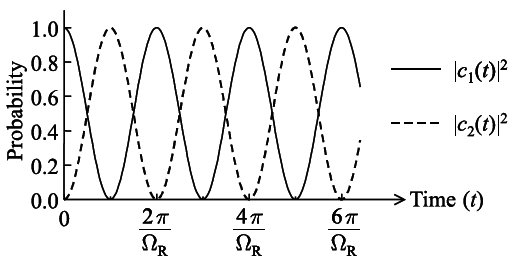
\includegraphics[width=0.6\textwidth]{figs/2022-05-22-12-48-32.png}
          \end{center} 
        强光场条件下,原子的激发形成拉比振荡. 在某些时间段,可出现粒子数反转. \\ 
\end{frame}

\begin{frame} 
\frametitle{}
\begin{center}
    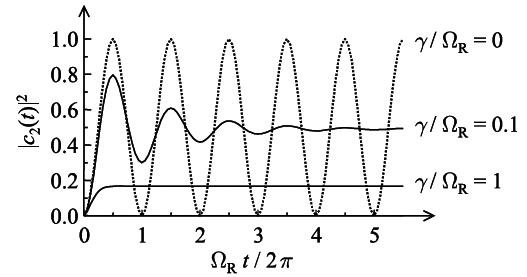
\includegraphics[width=0.6\textwidth]{figs/2022-05-22-13-14-30.png}
\end{center} 
        实验上,很难出现拉比振荡和粒子数反转, 因为\\ 
        (1) 拉比频率$\Omega_R = \frac{\left|\mathbf{E}_0\right|}{\hbar} X_{12}$与场强相关, 场强不大时, 拉比频率会大于原子的辐射寿命, 随机地自发辐射会消除相干叠加态, 导致振幅不断衰减. 因此,只有足够强的相干光场条件下,才能看到拉比振荡
    \end{frame}

\section{3. 全量子理论}

\begin{frame} 
\frametitle{哈密顿的构成}
     写出光-原子相互作用系统的哈密顿
     \[ H= H_a + H_o + H_{I}\]
\end{frame}

\begin{frame} 
\frametitle{}
    {\Bullet} 二能级系统(量子比特)的数学抽象 \\ 
    两能态分别表示为
    \[\rs{1}, \rs{2}\]
    构成正交归一完全基
    \[ \lr{i}{j}= \delta_{ij}, \quad \sum_i \rs{i} \ls{i} =1 ; \quad i,j=1,2\]
    态矢的展开
    \[\begin{aligned}
        \rs{\psi} &=\alpha\rs{1}+\beta\rs{2}, \qquad (|\alpha|^2+|\beta|^2=1)\\ 
        &=e^{i\gamma} \left(\cos\frac{\theta}{2}\rs{1}+e^{i\varphi} \sin\frac{\theta}{2}\rs{2}\right) \\
        &=\cos\frac{\theta}{2}\rs{1}+e^{i\varphi} \sin\frac{\theta}{2}\rs{2}
      \end{aligned}\]
    * 态矢由两个复数$\alpha,\beta$唯一确定, 也可由两个角度量$\theta, \varphi$ 唯一确定.
\end{frame}

\begin{frame} 
    \frametitle{} 
    ~\\
  在($r,\theta,\varphi$)坐标系中,由于$r\equiv 1$, 量子比对应$Bloch$球面上的一个点。
  \begin{center}
    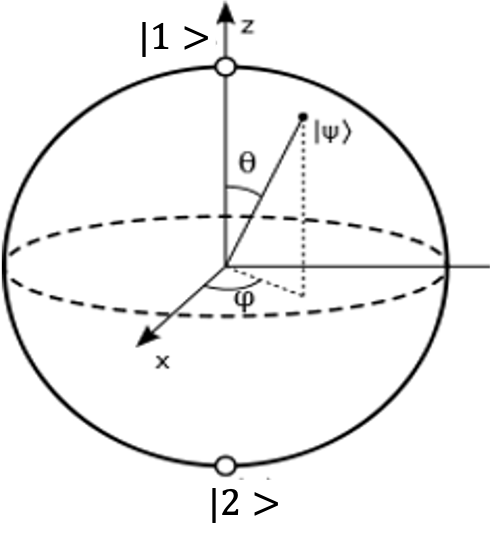
\includegraphics[width=0.4\textwidth]{figs/240.png}
\end{center} 
($\theta, \varphi$) 确定球面上的一唯点
\end{frame}

\begin{frame} 
    \frametitle{}
    因此, 
    \[\rs{\psi} =\alpha\rs{1}+\beta\rs{2} = \cos\frac{\theta}{2}\rs{1}+e^{i\varphi} \sin\frac{\theta}{2}\rs{2}\] 
    态函数展开系数构成矩阵表示\\
   \[
    \begin{matrix} 
    \rs{\psi} =\begin{pmatrix}
            \alpha\\
            \beta
    \end{pmatrix} =\begin{pmatrix}
        \cos\frac{\theta}{2}\\
        e^{i\varphi} \sin\frac{\theta}{2}
    \end{pmatrix}
    &    
    \rs{1} 
    =\begin{pmatrix}
        1\\
        0
    \end{pmatrix}
    &
    \rs{2} 
    =\begin{pmatrix}
        0\\
        1
    \end{pmatrix}
    \end{matrix}    
    \]
密度矩阵定义于外积:
 \[ \rho =\rl{\psi}{\psi} = \begin{pmatrix}
    \alpha\\
    \beta
\end{pmatrix} \begin{pmatrix}
    \alpha^* & \beta^*
\end{pmatrix}  = \begin{pmatrix}
    \alpha \alpha^*   &  \alpha \beta^* \\
    \alpha^* \beta   & \beta \beta^* 
\end{pmatrix} \]
 是一个$2\times 2$的矩阵
\end{frame}

\begin{frame} 
    \frametitle{}
    泡利矩阵是$2\times 2$空间的正交归一完全集 \\
    密度矩阵在这个完全集上的展开
    \[\begin{aligned}
        \rho =\rl{\psi}{\psi} 
    &=
    \begin{pmatrix}
        \cos\frac{\theta}{2}\\
        e^{i\varphi} \sin\frac{\theta}{2}
    \end{pmatrix}
    \begin{pmatrix}
        \cos\frac{\theta}{2} & e^{i\varphi} \sin\frac{\theta}{2}
    \end{pmatrix}
 \\
    &= \frac{1}{2}I +\frac{1}{2}\sin\theta\cos\varphi\sigma_x +\frac{1}{2}\sin\theta\sin\varphi\sigma_y+ \frac{1}{2}\cos\theta\sigma_z 
\end{aligned}\]
式中,泡利矩阵为
\[
I= \begin{pmatrix}
    1 & 0 \\
    0 & 1 
\end{pmatrix}, \quad
\sigma_x =
\begin{pmatrix}
    0 & 1 \\
    1 & 0 
\end{pmatrix}, \quad
\sigma_y =
\begin{pmatrix}
    0 & -i \\
    i & 0 
\end{pmatrix}, \quad
\sigma_z =
\begin{pmatrix}
    1 & 0 \\
    0 & -1 
\end{pmatrix}
\]
\end{frame}

\begin{frame} 
\frametitle{}
{\Bullet}二能级原子系统哈密顿的矩阵表示 \\ 
  定义$\hbar\omega= E_2-E_1, \quad  E_1+ E_2= 0 $
   \[\begin{aligned}
    H_a &= \begin{pmatrix}
        E_2 & 0\\ 
        0 & E_1 
     \end{pmatrix} \\
     &= \frac{E_2+E_1}{2} \begin{pmatrix}
        1 & 0\\ 
        0 & 1 
     \end{pmatrix} 
      + \frac{1}{2}\hbar \omega  \begin{pmatrix}
        1 & 0\\ 
        0 & -1 
     \end{pmatrix} \\
      &= \frac{1}{2}\hbar \omega \sigma_z  \\ 
      &= \hbar \omega S_z
    \end{aligned} \]   
\end{frame}

\begin{frame} 
\frametitle{}
   对应泡利算符:
    \[\begin{aligned}
        \sigma_z &=  (\rs{2} \ls{2}-\rs{1} \ls{1})\\ 
        \sigma_{+} &= \rs{2} \ls{1} \\ 
        \sigma_{-} &= \rs{1} \ls{2} \\ 
        \sigma_x &= (\sigma_{+}+ \sigma_{-}) \\ 
        \sigma_y &= \frac{1}{i}(\sigma_{+}- \sigma_{-}) \\ 
        S_i & =\frac{1}{2} \sigma_i, (i=x,y,z)
    \end{aligned} \]    
\end{frame}

\begin{frame} 
\frametitle{}
{\Bullet} 光场哈密顿采用全量子描述
\[ H_o = \sum_k \hbar \omega_k (a^{\dagger} _k a_k+\frac{1}{2})\]
对于单模光场
\[ H_o =  \hbar \omega_0 (a^{\dagger}  a + \frac{1}{2})\]
\end{frame}

\begin{frame} 
\frametitle{}
{\Bullet} 相互作用哈密顿   
\[ \begin{aligned}
    H_{I} & =  - \mathbf{d}\cdot \mathbf{E}(t)\\
    &= e\mathbf{r} \cdot \mathbf{E}(t) \\
    \mathbf{d} & = \mathbf{d}\rs{1}\ls{2}  + \mathbf{d}\rs{2}\ls{1} \\ 
    &= \mathbf{d}_{12} (\sigma_+ + \sigma_-) \\ 
    \mathbf{E}(\mathbf{r}) &= \sum_k \mathbf{e}_k \sqrt{ \frac{\hbar\omega_k}{2 \epsilon_0 V}} [{a}_k e^{i \mathbf{k}\cdot \mathbf{r}} + {a}^{\dagger} _k e^{-i \mathbf{k}\cdot \mathbf{r}} ] \\ 
    H_{I} & = \sum_k  \hbar g_k ({a}_k e^{i \mathbf{k}\cdot \mathbf{r}} + {a}^{\dagger} _k e^{-i \mathbf{k}\cdot \mathbf{r}} )(\sigma_+ + \sigma_-) 
\end{aligned}\] 
式中 $g$, 称为光场与原子的耦合常数,也称单光子拉比频率,偶极矩近似下为 
\[ g_k = \sqrt{ \frac{\omega_k}{2  \epsilon_0 \hbar V}} e \mathbf{r}\cdot\mathbf{e}_k \]
\end{frame}

\begin{frame} 
\frametitle{}
     \[ H_{I}  = \sum_k  \hbar g_k ({a}_k e^{i \mathbf{k}\cdot \mathbf{r}} + {a}^{\dagger} _k e^{-i \mathbf{k}\cdot \mathbf{r}} )(\sigma_+ + \sigma_-) \]
     产生四项
     \[ {a}^{\dagger} \sigma_+, \quad {a}^{\dagger} \sigma_-, \quad {a} \sigma_+, \quad {a} \sigma_- \]
     第一项和第四项为零
     \[ H_{I}  = \sum_k  \hbar g_k ({a}_k \sigma_+ e^{i \mathbf{k}\cdot \mathbf{r}} + {a}^{\dagger} _k \sigma_- e^{-i \mathbf{k}\cdot \mathbf{r}} )\]
     对于单模共振光场(简化 $\mathbf{r}=0$ )
     \[ H_{I} = \hbar g (a\sigma_+  +  a ^{\dagger} \sigma_{-} )\]
     式中,
     \[ g = \sqrt{ \frac{\omega}{2  \epsilon_0 \hbar V}} e \mathbf{r}\cdot\mathbf{e} \]
\end{frame}

\begin{frame} 
    \frametitle{}
        小结: 光与原子相互作用系统的哈密顿
             \[ H= \frac{1}{2}\hbar \omega \sigma_z + \sum_k \hbar \omega_k (a^{\dagger} _k a_k+\frac{1}{2}) + \sum_k \hbar g_k ( a_k \sigma_++  a_k ^{\dagger} \sigma_{-} )\]
        对于单模光场 (JC model)
    \[\begin{aligned}
        H &= \frac{1}{2}\hbar \omega \sigma_z + \hbar \omega_0 (a^{\dagger}  a +\frac{1}{2}) + \hbar g ( a \sigma_+ + a ^{\dagger} \sigma_{-}) 
    \end{aligned} \] 
    $Ficek$的书中写成了"自旋"算符的形式 
    \[\begin{aligned}
        H &= \hbar \omega S_z + \hbar \omega_0 (a^{\dagger}  a +\frac{1}{2}) - \frac{1}{2} i \hbar g (S^{+} a - S^{-} a ^{\dagger})
    \end{aligned} \]
    注意:与量子力学中的自旋算符小有差别 
    \[ S_i =\frac{\hbar}{2} \sigma_i, (i=x,y,z)\]
    \end{frame}

\begin{frame} 
    \frametitle{态函数}
        光与原子相互作用系统的态函数可以写成
        \[ \psi= \rs{n_o, n_a} \]
        式中 $n_o$,描述光场的数态, $n_a= 0$, or $1$, 描述原子的二个能级. \\ 
        对于无相互作用体系($g=0$)
        \[ \psi= \rs{n_o, n_a} = \rs{n_o}\otimes \rs{n_a} =\rs{n_o n_a} \]
        光与原子的两个态函数相互独立地演化. \\ 
        有相互作用时($g \not = 0$), 两体系的态函数存在关联!\\ 
    \end{frame}

    \begin{frame} 
    \frametitle{}
    {\Bullet} 对于共振吸收: $\Delta = \omega - \omega_0 =0 $
    设初态为 \[ \psi(0)= \rs{n, 1} \]
    则原子吸收一个光子后的状态为 \[ \psi(t)= \rs{n-1, 2} \]
    设初态为 \[ \psi(0)= \rs{n-1, 2} \]
    则原子放出一个光子后的状态为 \[ \psi(t)= \rs{n, 1} \]
    这两个态是能量简并的. \\
    对于非共振吸收: $\Delta = \omega - \omega_0 \not = 0 $
    则上述态的能量是非简并的. 
    \end{frame}

    \begin{frame} 
    \frametitle{}
    {\Bullet} 通常,体系处于叠加态
        \[ \rs{\psi(t)}= c_{1,n}(t) \rs{n, 1} + c_{2,n}(t) \rs{n-1, 2}  \]
    ~\\  
    波函数随时间的演化服从薛定谔方程
    \[ i \hbar \frac{\partial \psi(t)}{\partial t} = H \psi(t) \]
    \end{frame}

    \begin{frame} 
    \frametitle{解方程}
    代入 $H$ 和 $\psi(t)$\\  
    先处理方程的左边 
  \[ \begin{aligned}
    i \hbar \frac{\partial \psi(t)}{\partial t} & = H \psi(t)  \\
    i \hbar \frac{\partial }{\partial t} [c_{1,n}(t) \rs{n, 1} + c_{2,n}(t) \rs{n-1, 2}]& = H \psi(t)  \\
    i \hbar [\frac{\partial }{\partial t}c_{1,n}(t) \rs{n, 1} + \frac{\partial }{\partial t}c_{2,n}(t) \rs{n-1, 2}]& = H \psi(t)
  \end{aligned}\]      
    \end{frame}

    \begin{frame} 
    \frametitle{}
         再处理方程的右边
         \[ \begin{aligned}
            H \psi(t)= &[\hbar \omega S_z + \hbar \omega_0 (a^{\dagger}  a +\frac{1}{2}) - \frac{1}{2} i\hbar g (S^{+} a - S^{-} a ^{\dagger}  )] \psi(t) \\
          \end{aligned}\] 
        考虑共振的情况
        \[ \begin{aligned}
            \hbar \omega S_z \psi(t) &= \hbar \omega S_z [c_{1,n}(t) \rs{n, 1} + c_{2,n}(t) \rs{n-1, 2}] \\ 
            &= \hbar \omega [ -\frac{1}{2}c_{1,n}(t) \rs{n, 1} + \frac{1}{2}c_{2,n}(t) \rs{n-1, 2}] \\
           \hbar \omega_0 (a^{\dagger}  a +\frac{1}{2}) \psi(t) 
           &= \hbar \omega_0 (a^{\dagger}  a +\frac{1}{2}) [c_{1,n}(t) \rs{n, 1} + c_{2,n}(t) \rs{n-1, 2}] \\ 
        &=\hbar \omega_0 [ (n +\frac{1}{2})c_{1,n}(t) \rs{n, 1} + (n -\frac{1}{2})c_{2,n}(t) \rs{n-1, 2}]  \\ 
        - \frac{1}{2} i\hbar g (S^{+} a - S^{-} a ^{\dagger}  ) \psi(t) &= - \frac{1}{2} i\hbar g (S^{+} a - S^{-} a ^{\dagger}  )[c_{1,n}(t) \rs{n, 1} + c_{2,n}(t) \rs{n-1, 2}] \\ 
        &= - \frac{1}{2} i\hbar g [c_{1,n}(t) \sqrt{n} \rs{n-1, 2} - c_{2,n}(t) \sqrt{n} \rs{n, 1}] 
          \end{aligned}\]
    \end{frame}

    \begin{frame} 
    \frametitle{}
    下式左乘 $\ls{1,n}$
    \[ \begin{aligned}
        i \hbar [\frac{\partial }{\partial t}c_{1,n}(t) \rs{n, 1} + &\frac{\partial }{\partial t}c_{2,n}(t) \rs{n-1, 2}] = H \psi(t) \\ 
        i \hbar \frac{\partial }{\partial t}c_{1,n}(t) &= \ls{1,n} H \psi(t) \\ 
        &= -\hbar \omega \frac{1}{2}c_{1,n}(t) + \hbar \omega_0 (n +\frac{1}{2})c_{1,n}(t) + \frac{1}{2} i\hbar g \sqrt{n} c_{2,n}(t) \\ 
        &=  \hbar \omega n c_{1,n}(t) + \frac{1}{2} i\hbar g \sqrt{n} c_{2,n}(t)
      \end{aligned}\] 
      下式左乘 $\ls{2,n-1}$
      \[ \begin{aligned}
          i \hbar [\frac{\partial }{\partial t}c_{1,n}(t) \rs{n, 1} +& \frac{\partial }{\partial t}c_{2,n}(t) \rs{n-1, 2}] = H \psi(t) \\ 
          i \hbar \frac{\partial }{\partial t}c_{2,n}(t) &= \ls{2,n-1} H \psi(t) \\ 
          &=  \hbar \omega n c_{2,n}(t) - \frac{1}{2} i\hbar g \sqrt{n} c_{1,n}(t) 
        \end{aligned}\] 
    \end{frame}

    \begin{frame} 
    \frametitle{}
         联立, 得方程组
        \[ \begin{cases}
            i \hbar \frac{\partial }{\partial t}c_{1,n}(t) &=\hbar \omega n c_{1,n}(t) + \frac{1}{2} i\hbar g \sqrt{n} c_{2,n}(t) \\ 
            &~ \\ 
            i \hbar \frac{\partial }{\partial t}c_{2,n}(t) &=\hbar \omega n c_{2,n}(t) - \frac{1}{2} i\hbar g \sqrt{n} c_{1,n}(t) 
        \end{cases} \]
        给定初始条件$c_{1,n}(0) = \left\langle 1,n|\psi(0) \right\rangle ,c_{2,n}(0)=\left\langle 2,n|\psi(0) \right\rangle$, 方程可求解 
    \[\begin{cases}
        c_{1,n}(t) &= \frac{1}{2} e^{ i (n \omega t)} \left\{ [ -i c_{2,n}(0) - c_{1,n}(0)] e^{-\frac{1}{2} i \Omega t}  + [ -i c_{2,n}(0) + c_{1,n}(0)] e^{\frac{1}{2} i \Omega t}\right\} \\
        ~ \\
        c_{2,n}(t) &= \frac{1}{2} e^{- i (n \omega t)} \left\{ [ i c_{2,n}(0) - c_{1,n}(0)] e^{\frac{1}{2} i \Omega t}  + [ i c_{2,n}(0) + c_{1,n}(0)] e^{-\frac{1}{2} i \Omega t}\right\} \\
    \end{cases} \]
    式中 $\Omega = g \sqrt{n}$, 是拉比频率
    \end{frame}

    \begin{frame} 
    \frametitle{分析}
        (1) 激发态原子的数目 \\ 
        {\Bullet}考虑初始态为所有原子都处于基态$\rs{1}$, 光场处于数态$\rs{n_0}$
        \[ \rs{\psi(0)} = \rs{n_0, 1}\]
        对应的初始条件为:
    \[\begin{aligned}
        c_{1,n}(0) &= \left\langle 1,n|\psi(0)\right\rangle \\  
        &=  \left\langle 1,n| n_0, 1\right\rangle\\ 
        &= \delta_{n,n_0} \\ 
        c_{2,n}(0) &= \left\langle 2,n|\psi(0)\right\rangle \\  
        &=  \left\langle 2,n| n_0, 1\right\rangle\\ 
        &= 0
    \end{aligned} \]
    代回解函数
    \end{frame}

    \begin{frame} 
    \frametitle{}
    得:
    \[\begin{aligned}
             \left|c_{2,n}\right|^2 &= \sin^2 (\frac{1}{2}\Omega t) \delta_{n,n_0} \\ 
             P_2(t) &= \sum_n \left|c_{2, n}\right|^2  \\ 
             &= \sin ^2 (\frac{1}{2}\Omega t) 
    \end{aligned} \]
    说明, 原子被共振激发的概率呈现周期振荡行为, 振荡的频率是拉比频率.  \\ 
    \end{frame}

    \begin{frame} 
    \frametitle{}
    (2)崩塌和复兴效应 \\
    {\Bullet}考虑光场不处于数态, 而是数态的叠加态, 比如相干态, 而原子处于基态
    \[ \rs{\psi(0)} = \rs{\alpha, 1}\] 
    对应的初始条件为:
    \[\begin{aligned}
        c_{1,n}(0) &= \left\langle 1,n|\psi(0)\right\rangle \\  
        &=  \left\langle 1,n| \alpha, 1\right\rangle\\ 
        &= \left\langle n| \alpha \right\rangle \\
        &= \left\langle n \left| e^{-\frac{1}{2}|\alpha|^2}  \sum_{n=0} ^{+\infty}  \frac{\alpha^n}{\sqrt{n!}} \right| n \right\rangle\\ 
        &= e^{-\frac{1}{2}|\alpha|^2} \sum_{n=0} ^{+\infty}  \frac{\alpha^n}{\sqrt{n!}} \\
        c_{2,n}(0) &= 0
    \end{aligned} \]
    \end{frame}

    \begin{frame} 
    \frametitle{}
         同理,得
         \[\begin{aligned}
            P_2(t) &= \sum_n  \frac{\overline{n}^n}{\sqrt{n!}} e^{-\overline{n}} \sin ^2 (\frac{1}{2} \sqrt{n} g t) 
   \end{aligned} \]
      \begin{center}
           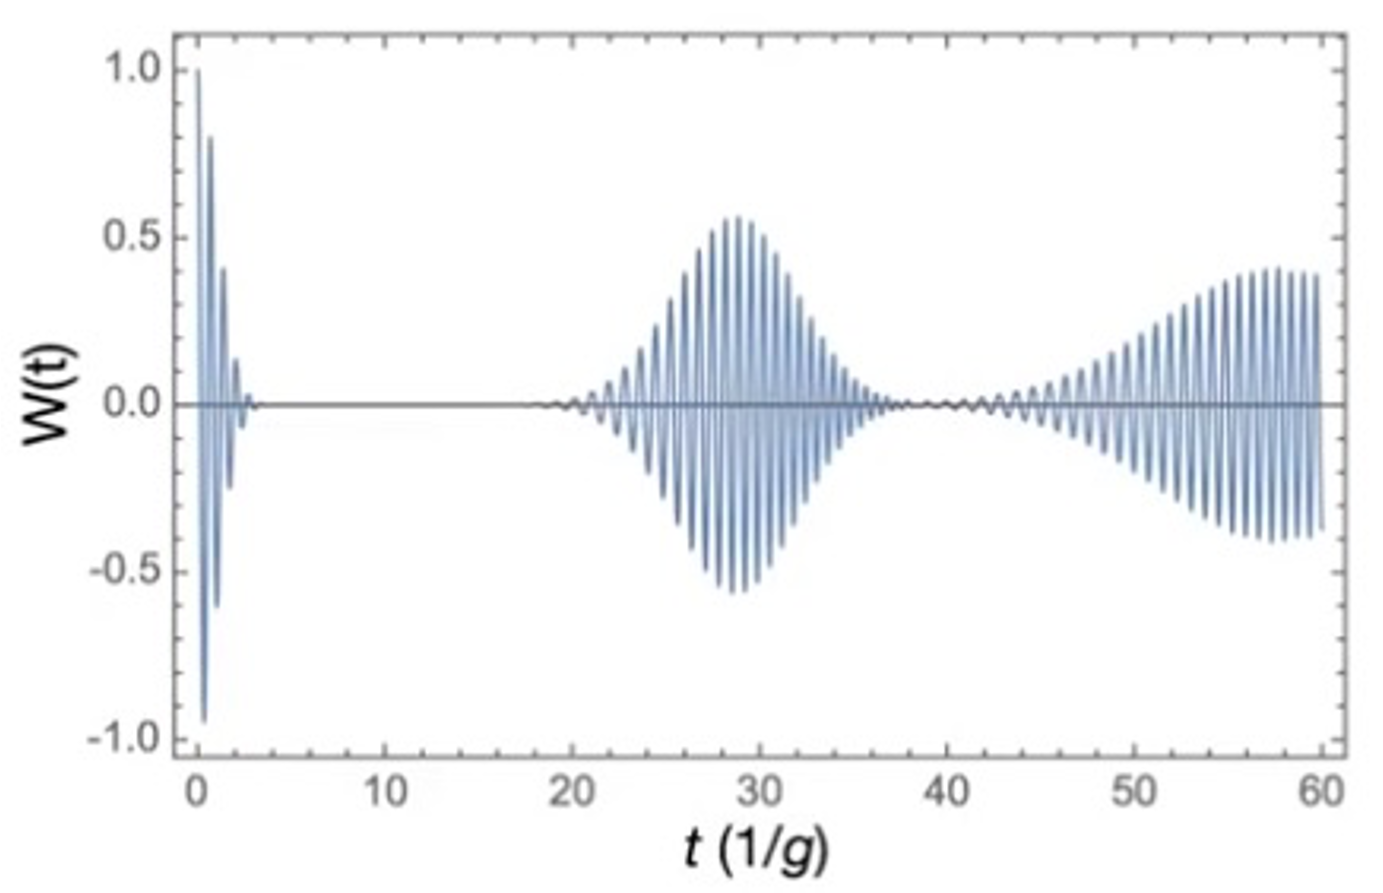
\includegraphics[width=0.5\textwidth]{figs/29.png}
      \end{center}
      拉比振荡呈现量子化现象
    \end{frame}

\begin{frame} 
\frametitle{}
    分析:
\[\begin{aligned}
    P_2(t) &= \sum_n  \frac{\overline{n} ^n}{\sqrt{n!}} e^{-\overline{n}} \sin ^2 (\frac{1}{2} \sqrt{n} g t) \\ 
    &= \frac{1}{2} \left[ 1 - \sum_n  \frac{\overline{n}^n}{\sqrt{n!}} e^{-\overline{n}} \cos (\sqrt{n} g t) \right] \\ 
    &= \frac{1}{2} \left[ 1 - \sum_n  \frac{\overline{n}^n}{\sqrt{n!}} e^{-\overline{n}} Re(e^{i\sqrt{n} g t}) \right] \\ 
    &= \frac{1}{2} \left[ 1 - Re(e^{i\sqrt{\overline{n}} g t} D(t)) \right] \\ 
\end{aligned} \] 
式中存在两种振荡
\[ e^{i\sqrt{\overline{n}} g t}, \quad D(t) =  \sum_n  \frac{\overline{n}^n}{\sqrt{n!}} e^{-\overline{n}} e^{i(\sqrt{n}-\sqrt{\overline{n}}) g t}\]
前者快频振荡, 后者慢频振荡. 
\end{frame}

\begin{frame} 
\frametitle{}
慢频振荡项有两种相位, \\ 
     (1) 当 
     \[\sqrt{n}-\sqrt{\overline{n}}> 0\]
    是负频. \\ 
    (2) 当 
    \[\sqrt{n}-\sqrt{\overline{n}}< 0\]
    是正频.\\ 
   不同频率的干涉会导致强度先趋零(崩塌), 然后再变大(复兴).
\end{frame}

\begin{frame} 
\frametitle{}
    设导致的光子数变数为 $\Delta n$, 而两相的相差为$\pi$, 有: 
    \[\left(\sqrt{\overline{n}+\frac{1}{2}\Delta n}-\sqrt{\overline{n}}\right) gt = \left(\sqrt{\overline{n}-\frac{1}{2}\Delta n}-\sqrt{\overline{n}}\right) gt + \pi  \]
    \[ \to  t_c = \frac{2\pi}{g} \frac{\sqrt{\overline{n}}}{\Delta n}\]
    对于泊松光场,
    \[ t_c = \frac{2\pi}{g} \]
    两临近数态相差变为 $2\pi$时, 复兴开始
    \[ \left(\sqrt{\overline{n} +1} -\sqrt{\overline{n}}\right) gt = 2\pi \]
    \[ \to t_R= \frac{4\pi}{g}\sqrt{\overline{n}} \]
\end{frame}

\begin{frame} 
\frametitle{}
     两者的比值为
     \[ \frac{t_R}{t_c} = 2 \Delta n \]
     由于 $\Delta n\gg 1$, 等待复兴的时间要远长于崩塌所化的时间
\end{frame}
    %%%%%%%%%%%%%%%%%%%%%%%%%%%%%%%%%%%%%%%%%%%%%%%%%%%%%%%%%%%%%%%%%%%
    \begin{frame} 
        \frametitle{课外作业}
        \begin{enumerate}
            \item 试用 $JC-model$ 哈密顿形式,完成后面的计算过程
            \item 试估算崩塌的时间和复兴的时间
        \end{enumerate}
    \end{frame}
    %%%%%%%%%%%%%%%%%%%%%%%%%%%%%%%%%%%%%%%%%%%%%%%%%%%%%%%%%%%%%%%%%%%